\chapter{Diagrams}


\begin{figure}[t]
    \centering
    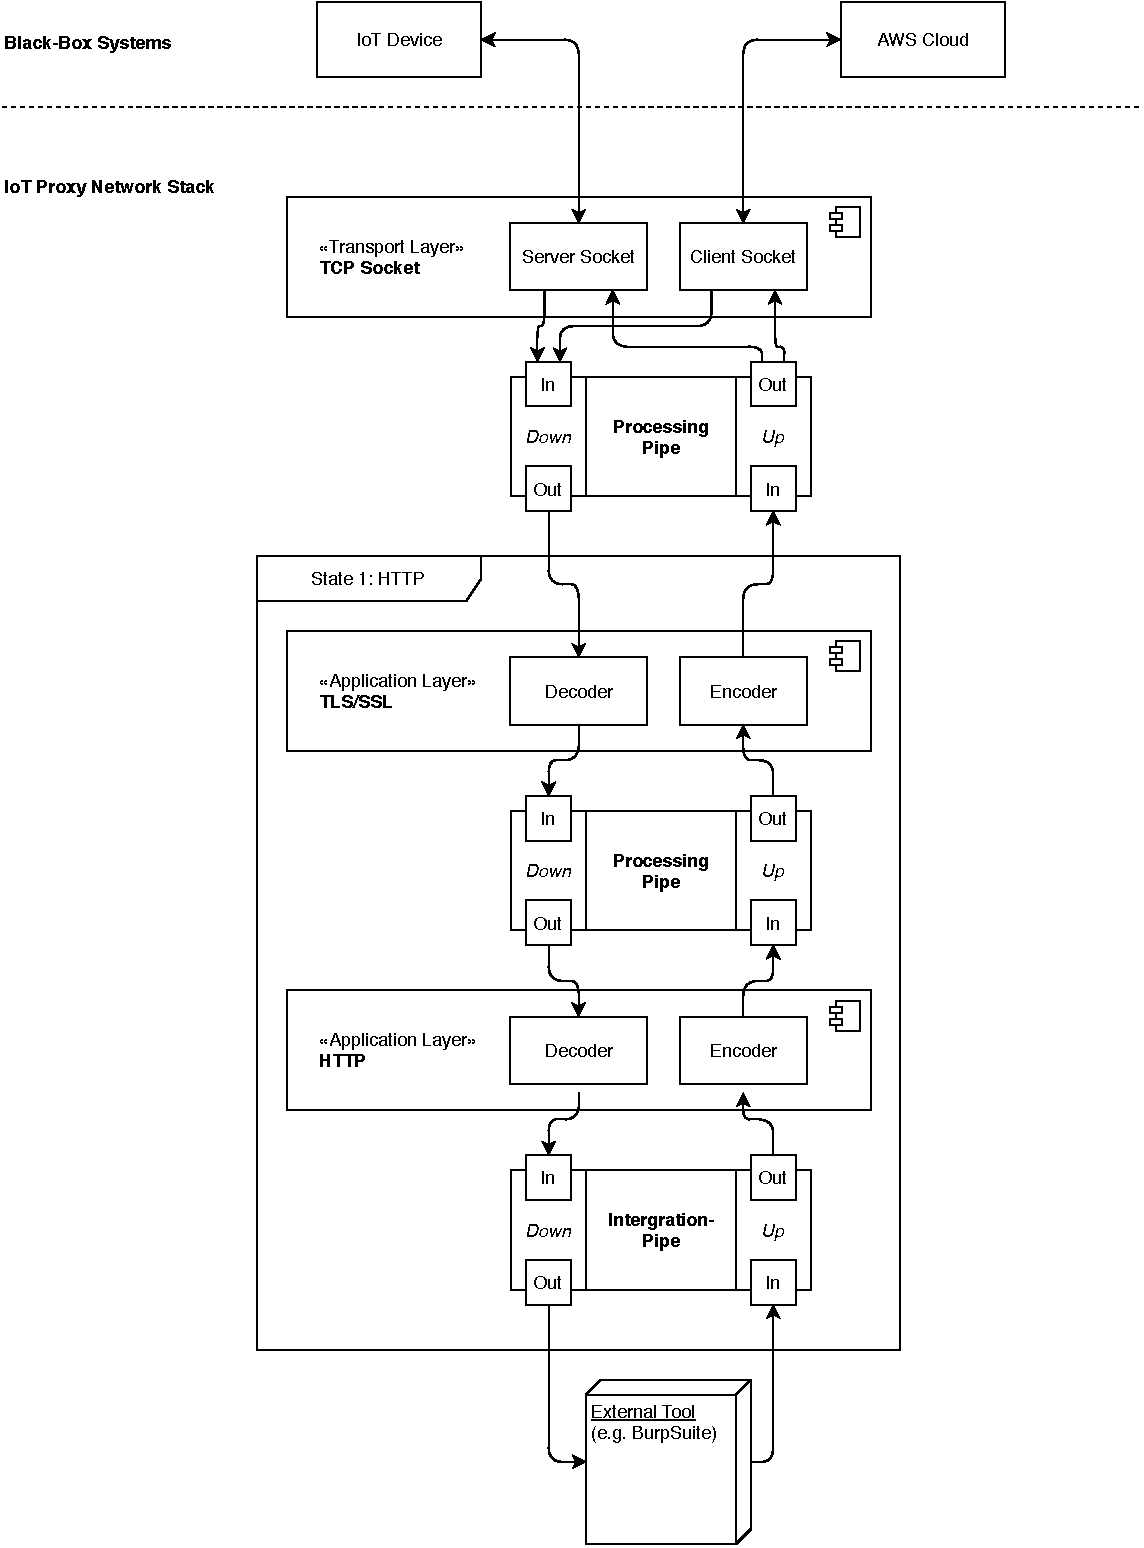
\includegraphics[width=14cm]{img/ch04/Architecture - PipesFilters 1.pdf}
    \captionof{figure}{\ac{AWS} \ac{IoT} Scenario - State 1: \ac{HTTP} Server}
    \label{fig:app-diag-pipesfilters-1}
\end{figure}

\begin{figure}[t]
    \centering
    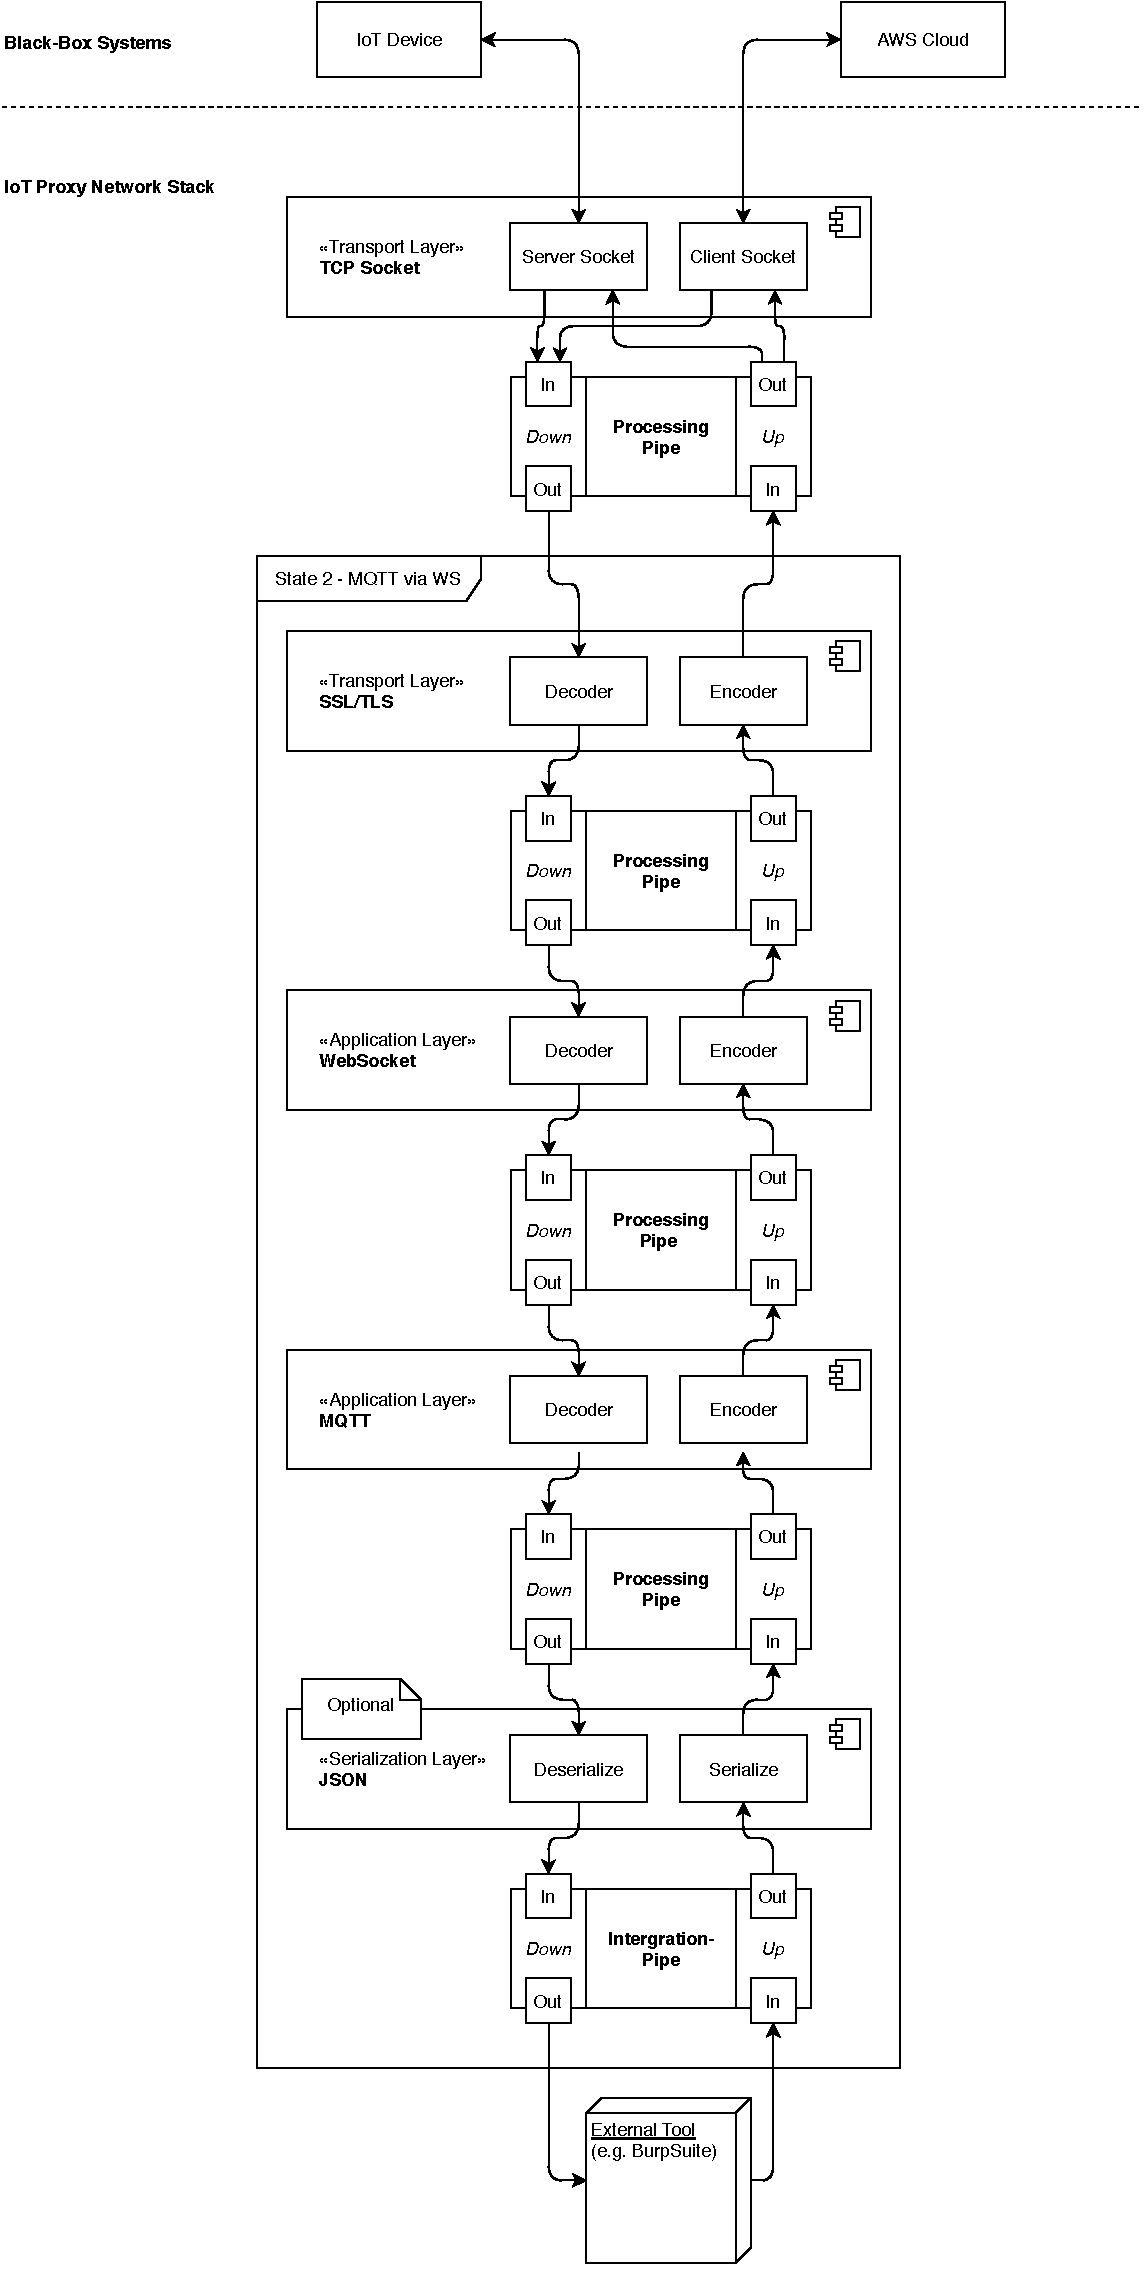
\includegraphics[width=12cm]{img/ch04/Architecture - PipesFilters 2.pdf}
    \captionof{figure}{\ac{AWS} \ac{IoT} Scenario - State 2: \ac{MQTT} via \ac{WS}}
    \label{fig:app-diag-pipesfilters-2}
\end{figure}

\begin{figure}[t]
    \centering
    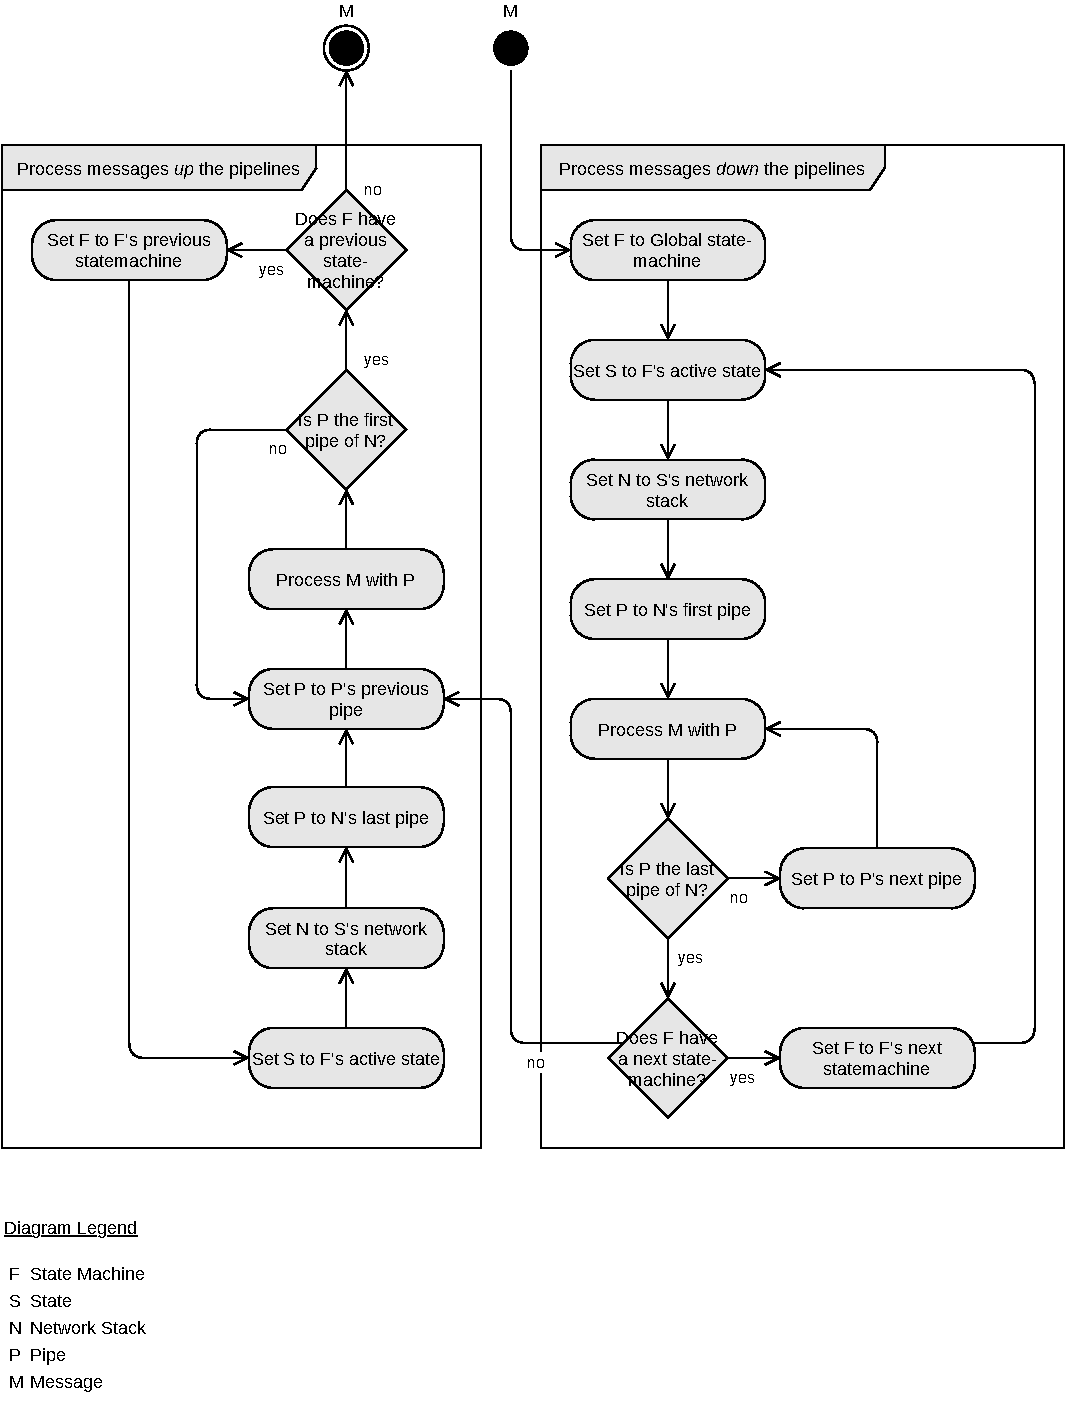
\includegraphics[width=14cm]{img/ch05/activity-nested-fsms.pdf}
    \captionof{figure}{Message processing through an architecture of nested \acp{FSM} and network stacks}
    \label{fig:app-activity-fsms}
\end{figure}

\begin{sidewaysfigure}[h]
    \centering
    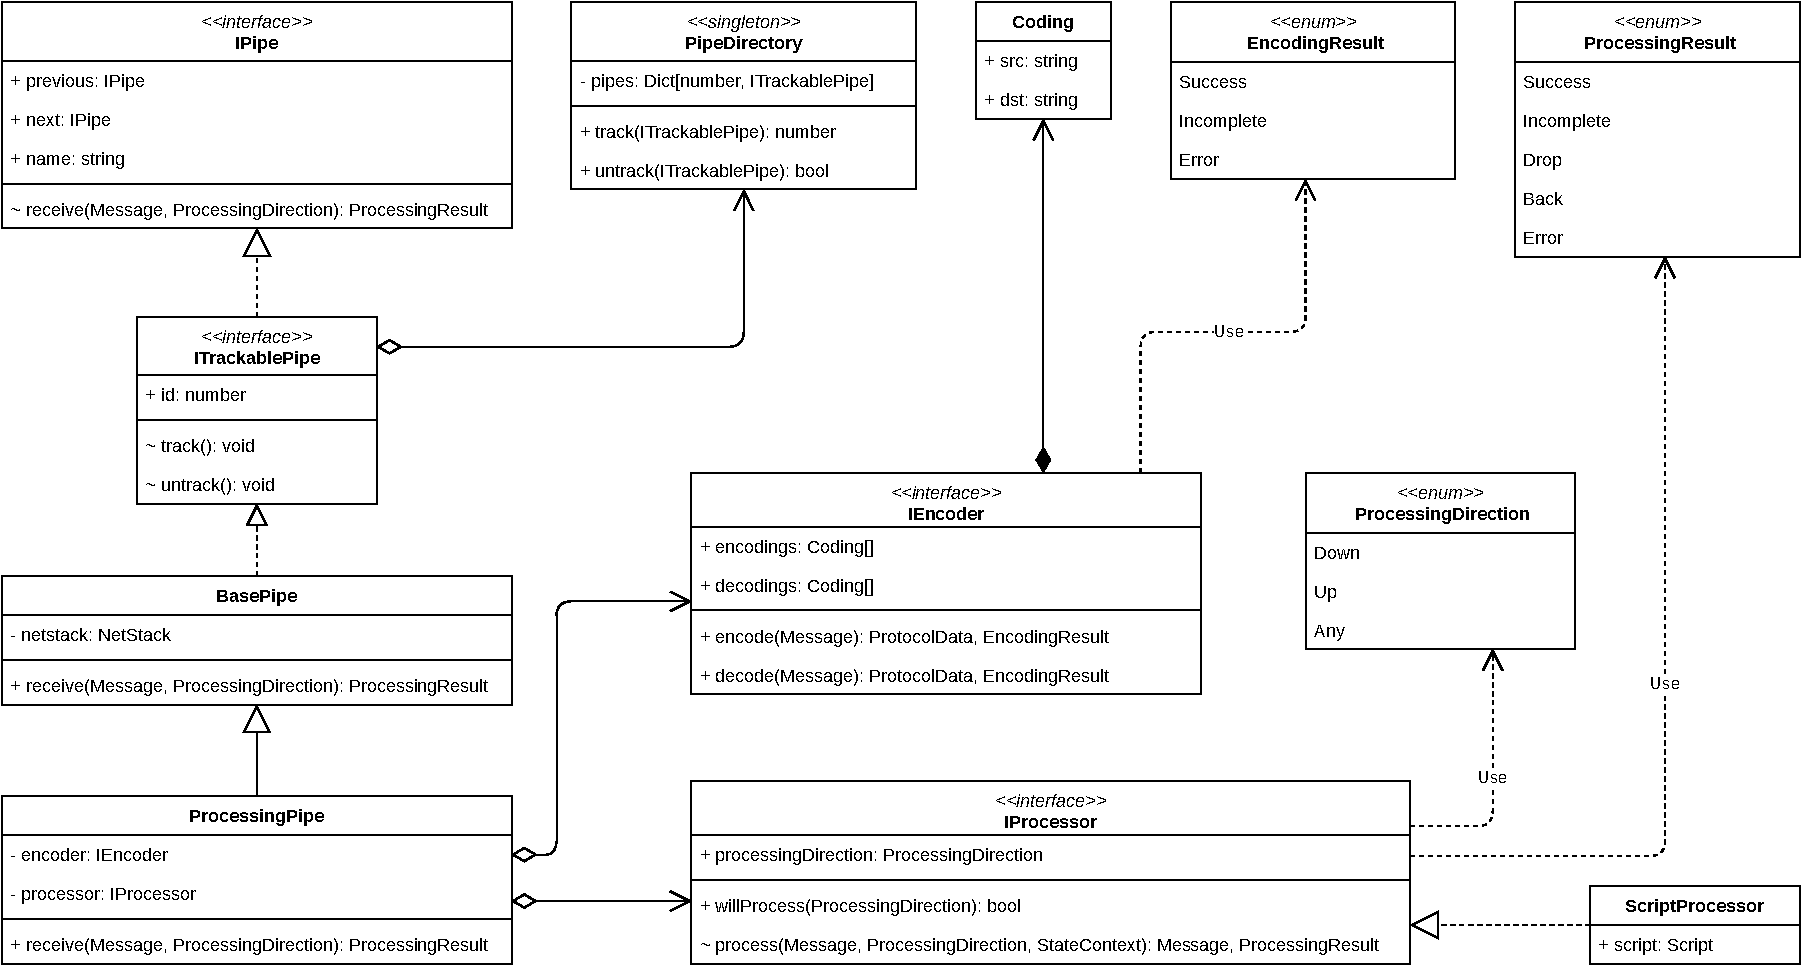
\includegraphics[height=12cm]{img/ch05/classes-2-pipes.pdf}
    \captionof{figure}{?} %TODO: Describe
    \label{fig:app-classes-2-pipes}
\end{sidewaysfigure}

\begin{figure}[h]
    \centering
    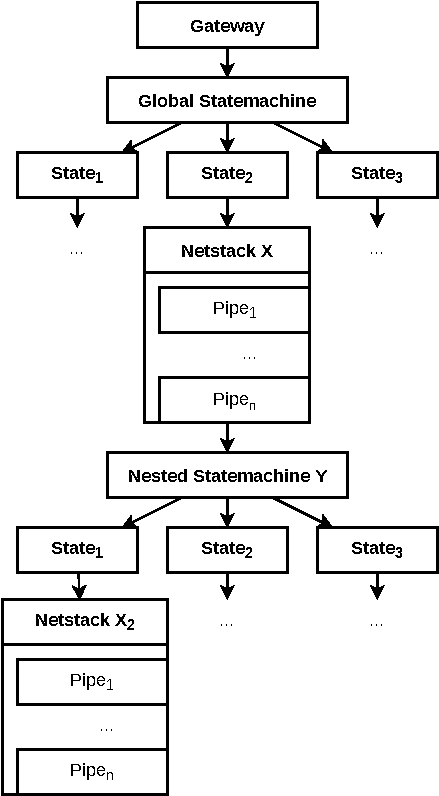
\includegraphics[height=12cm]{img/ch05/pipeline.pdf}
    \captionof{figure}{?} %TODO: Describe
    \label{fig:pipeline}
\end{figure}